% ****** Start of file apssamp.tex ******
%
%   This file is part of the APS files in the REVTeX 4.1 distribution.
%   Version 4.1r of REVTeX, August 2010
%
%   Copyright (c) 2009, 2010 The American Physical Society.
%
%   See the REVTeX 4 README file for restrictions and more information.
%
% TeX'ing this file requires that you have AMS-LaTeX 2.0 installed
% as well as the rest of the prerequisites for REVTeX 4.1
%
% See the REVTeX 4 README file
% It also requires running BibTeX. The commands are as follows:
%
%  1)  latex apssamp.tex
%  2)  bibtex apssamp
%  3)  latex apssamp.tex
%  4)  latex apssamp.tex
%
\documentclass[%
 reprint,
%superscriptaddress,
%groupedaddress,
%unsortedaddress,
%runinaddress,
%frontmatterverbose,
%preprint,
%showpacs,preprintnumbers,
%nofootinbib,
%nobibnotes,
%bibnotes,
 amsmath,amssymb,
 aps,
%pra,
%prb,
%rmp,
%prstab,
%prstper,
%floatfix,
]{revtex4-1}

\usepackage[utf8]{inputenc}
\usepackage[norsk]{babel}
\usepackage{graphicx}% Include figure files
\usepackage{dcolumn}% Align table columns on decimal point
\usepackage{bm}% bold math
\newcommand*\diff{\mathop{}\!\mathrm{d}}
\newcommand*\Diff[1]{\mathop{}\!\mathrm{d^#1}}
\usepackage{lipsum}
\usepackage{dsfont}
\usepackage{commath}
\usepackage[free-standing-units=true]{siunitx}

%ROMERSKE TALL med \rom
\makeatletter
\newcommand*{\rom}[1]{\expandafter\@slowromancap\romannumeral #1@}

\usepackage{physics}
\usepackage{caption}
\usepackage{varioref}
\usepackage{bm}
\usepackage{hyperref}% add hypertext capabilities
\usepackage[mathlines]{lineno}% Enable numbering of text and display math

\begin{document}
\title{Elastisitet}
\author{\textsc{Ivar Svalheim Haugerud}}
\affiliation{ Universitetet i Oslo}
\date{\today}

\begin{abstract}
\end{abstract}

\pacs{Valid PACS appear here}% PACS, the Physics and Astronomy
                             % Classification Scheme.
%\keywords{Suggested keywords}%Use showkeys class option if keyword
                              %display desired
\maketitle

%\tableofcontents

\section{Teori}
defleksjonen $h(m)$ til en bjelke, som støtter seg på to punkter med avstand $l$, som bærer en last på $mg$ i midten av bjelken gitt ved
\begin{equation}
  h(m) = \frac{mgl^3}{48EI}.\label{young}
\end{equation}
I dette uttrykket er $E$ elastisitetsmodulen og $I$ er arealtreghetsmomentet til bjelken, ikke massetreghetsmomentet som brukes i dynamikk. Arealtreghetsmomentet, også kalt andre arealmoment, er integralet over tversnittet til bjelken
\begin{equation}
  I = \int\int x^2 \diff y \diff x,
\end{equation}hvor bjelken strekker seg ut i $z$-retning, og lasten virker i $x$-retning. For eksperimentet vi skal gjøre kommer bjelken til å være en sylinder. Vi kan derfor beregne arealtreghetsmomentet til en sylinder med radius $R$. Vi beregner integralet i sylinderkoordinater, og har derfor multiplisert med jacobideterminanten, og brukt at $x = r\sin{\theta}$. Vi får
\begin{equation}
  I = \int_0^{2\pi} \int_0^R r^2\sin^2{\theta}r \diff r \diff \theta = \frac{\pi r^4}{4} = \frac{\pi d^4}{64},
\end{equation}der $d$ er diameteren. Setter vi dette inn i \eqref{young} får vi
\begin{equation*}
  h(m) = \frac{4mgl^3}{3\pi Ed^4}.
\end{equation*}
Siden vi er interesert i å måle elastisitetsmodulen til bjelken kan vi løse for likningen for $E$ for å få
\begin{equation}
  E = \frac{4mgl^3}{3\pi hd^4}. \label{young2}
\end{equation}
Under eksperimentet kommer vi til å finne $h(m)$, som vi forventer har en lineært forhold med lasten $m$
\begin{equation}
  h(m) = Am + B.
\end{equation}
Konstantleddet $B$ vil være tilnærmet lik null, og vi kan derfor erstatte $h/m$ med stigningstallet $A$ som vi vil beregne under målingene. Setter vi dette inn i \eqref{young2} får vi et uttrykk for elastisitetsmodulen til bjelken hvor vi kan måle alle de ukjente variablene
\begin{equation}
  E = \frac{4gl^3}{3\pi Ad^4}. \label{young3}
\end{equation}
Fra dette uttrykket kan vi beregne en verdi for elastisitetsmodulen.\\Vi ønsker å bruke en annen metode for å finne elastisitetsmodulen. Denne metoden for bestemmelse av E baserer seg på at utbredelseshastigheten $v$ for longitudinalbølger i en stav er gitt ved
\begin{equation*}
  v = \sqrt{\frac{E}{\rho}},\label{vel}
\end{equation*}
hvor $\rho$ er mediets tetthet. For å beregne $\rho$ kan vi måle massen og volumet til staven som er gitt av
\begin{equation}
  \rho = \frac{4M}{\pi L d^2}.
\end{equation}
Vi kan sette dette inn for $\rho$ i \eqref{vel} og løse for $E$, som gir oss
\begin{equation}
  E = \frac{4Mv^2}{\pi L d^2}.\label{elast}
\end{equation}
For å kunne beregne elastisitetsmodulen mangler vi bare utbredelseshastigheten i staven. Denne kan vi bestemme ved å måle verdien til frekvens $f$ og bølgelengden $\lambda$, som gir oss hastigheten ved sammenhengen
\begin{equation}
  v = \lambda f.\label{vlf}
\end{equation}
Både bølgelengde og frekvens kan bestemmes ved måling på en stående bølge i staven.
Det kan vises at ved frie longitudinelle svingninger i en homogen stav med lengde $L$ opphengt i midtpunktet og med frie ender, får vi stående bølger slik at
\begin{equation}
  L = \frac{n\lambda}{2},
\end{equation}
dette kan løses for $\lambda$, som gir oss
\begin{equation}
  \lambda = \frac{2L}{n},
\end{equation}
der $n$ er et oddetall $n = 1, 3, 5, ...$. Ved å slå staven i aksial retning dannes det flere egensvingninger i staven. Av disse stående bølgendene er det den med støst bølgelengde, $\lambda = 2L$, som blir sterkest. Denne bølgen vil også bli svakest dempet, og vil derfor etterhvert bli den dominerende bølgen i staven. Ved noen verdier for $L$ kan disse bølgene gi hørbar lyd. Vi kommer derfor til å bruke
\begin{equation}
  \lambda = 2L
\end{equation}i beregningen av elastisitetsmodulen. Setter vi dette inn for bølgelengden i \eqref{vlf} og får vi
\begin{equation}
  v = 2Lf,
\end{equation}som vi kan sette inn for utbredelseshastigheten i \eqref{elast} får vi
\begin{equation}
  E = \frac{16MLf^2}{\pi d^2}.\label{young5}.
\end{equation}
Ved å kunne måle de geometriske størrelsene til stangen og frekvensen når vi slår på den klarer vi å beregne elastisitetsmodulen på en ny måte.
\section{Metode}
\begin{figure*}
  \centering
  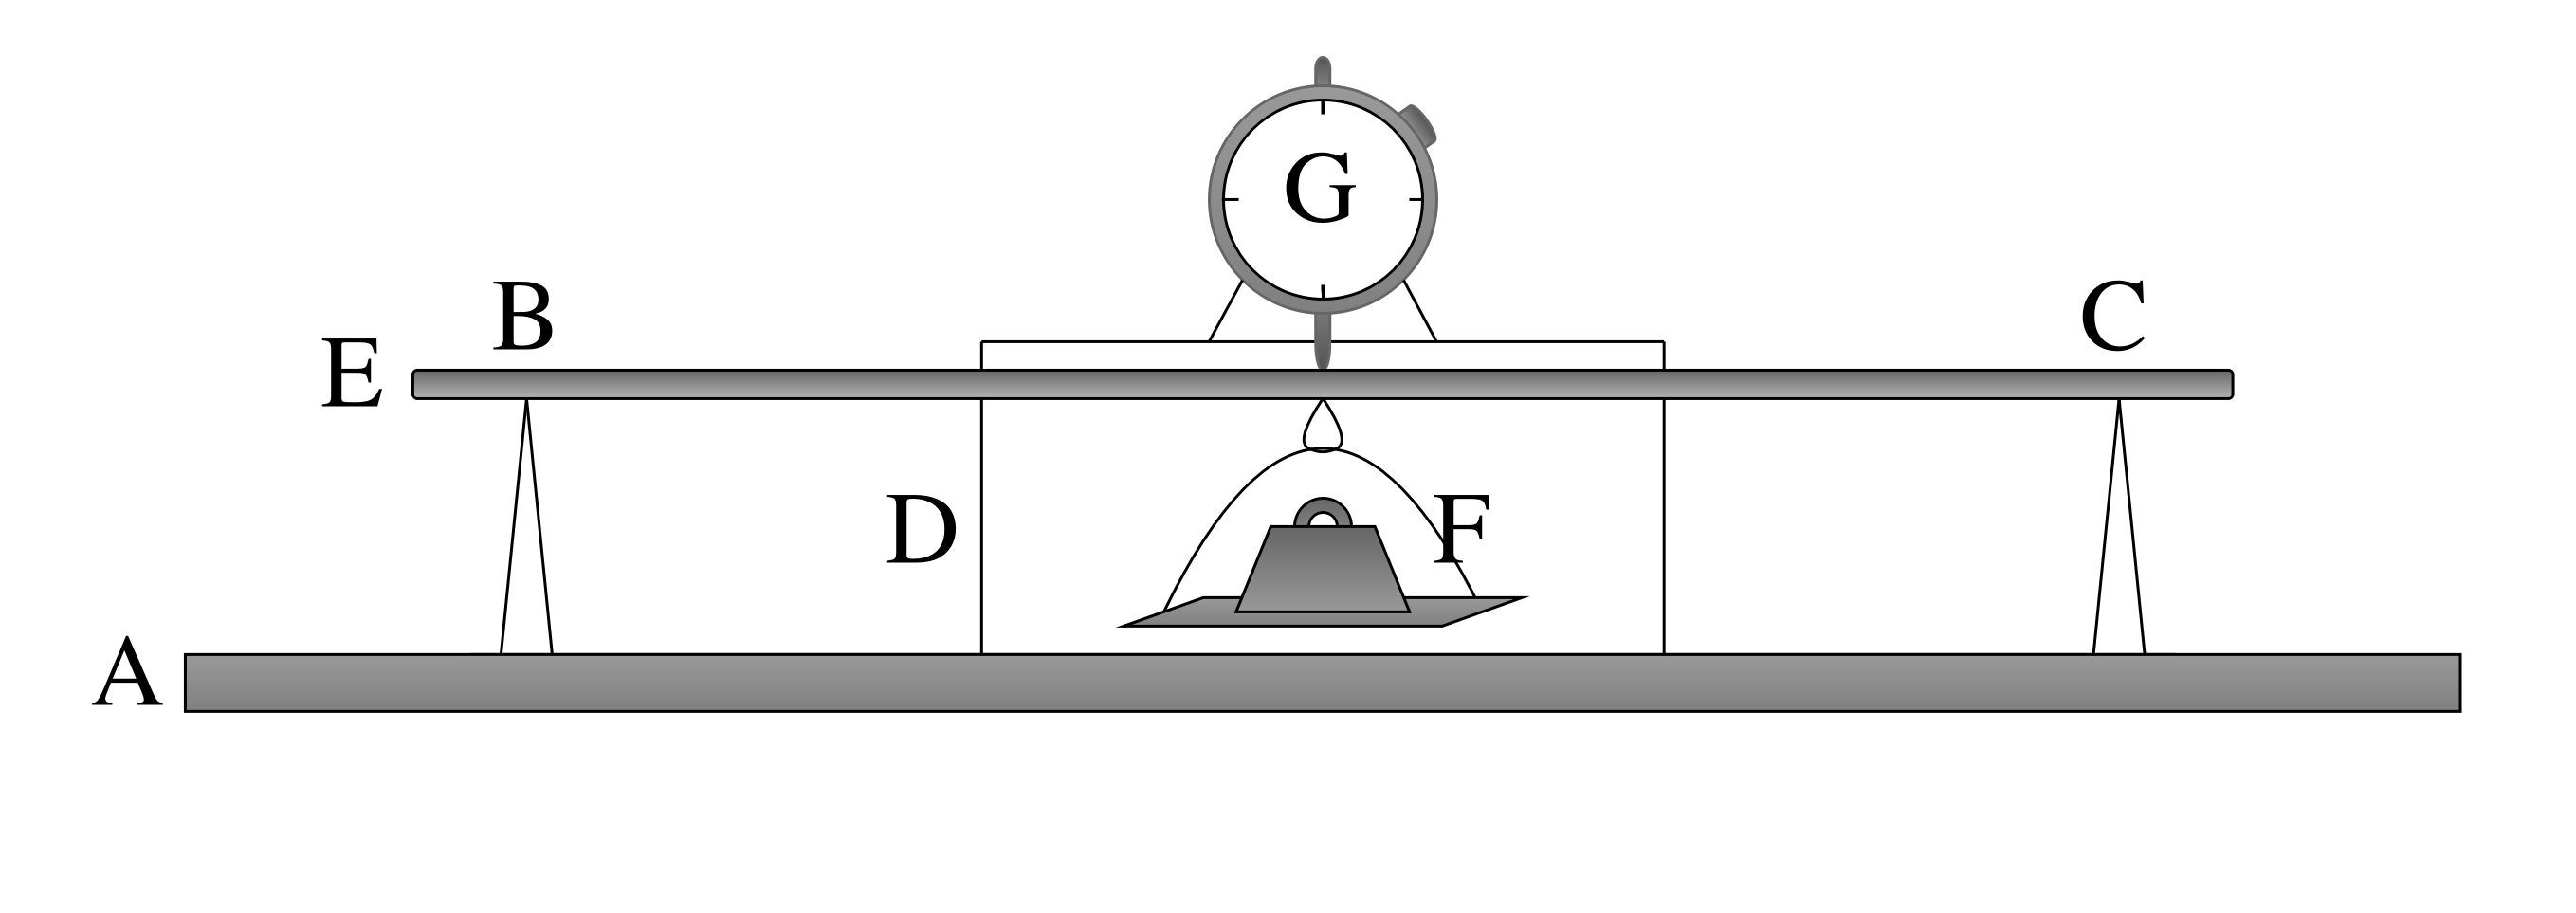
\includegraphics[scale=0.17]{oppsett.png}
  \caption{Eksperimentelt oppsett for målinger. Vi bruker en messingstang $E$ som hviler på to kniver $B$ og $C$. Midt på bjelken er det festet en flate $F$ hvor vi kan feste vekter, og vi kan måle avstanden den faller ned med måleuret $G$. Hele eksperimentet foregår på en plate $A$.}
  \label{eksperiment}
\end{figure*}
\begin{thebibliography}{9}
\bibitem{squires}
Squires, G.L. \emph{Practical Physics}, Cambridge University Press, 2001.
\bibitem{oppgave}
Fysisk institutt \emph{Elastisitet}, Universitetet i Oslo, februar 2018.
\end{thebibliography}

\end{document}
%
% ****** End of file apssamp.tex ******
